\documentclass[12pt]{article}
 
\usepackage[margin=0.75in]{geometry} 
\usepackage{amsmath,amsthm,amssymb}
\usepackage{physics}
\usepackage{nicematrix}
\usepackage{mathdots}
\usepackage{mathtools}
\usepackage{enumitem}
\usepackage{caption}
\usepackage{array}
\usepackage{float}
\usepackage{multirow}
\usepackage{tikz}
\usepackage[T1]{fontenc}
\usepackage[numbered,framed]{matlab-prettifier}
\usepackage{MnSymbol,wasysym}
\usepackage{hyperref}
\usepackage{filecontents}
\def\firstcircle{(90:4cm) circle (4.5cm)}
\def\secondcircle{(200:3cm) circle (4.5cm)}
\def\thirdcircle{(340:3cm) circle (4.5cm)}

\newcommand{\N}{\mathbb{N}}
% Bold for vectors and matrices
\newcommand\vect[1]{\mathbf{#1}}
\newcommand{\Z}{\mathbb{Z}}
\renewcommand{\theenumi}{\alph{enumi}}

\definecolor{dkgreen}{rgb}{0,0.6,0}
 
\newenvironment{theorem}[2][Theorem]{\begin{trivlist}
\item[\hskip \labelsep {\bfseries #1}\hskip \labelsep {\bfseries #2.}]}{\end{trivlist}}
\newenvironment{lemma}[2][Lemma]{\begin{trivlist}
\item[\hskip \labelsep {\bfseries #1}\hskip \labelsep {\bfseries #2.}]}{\end{trivlist}}
\newenvironment{exercise}[2][\large Exercise]{\begin{trivlist}
\item[\centering \Large \hskip \labelsep {\bfseries #1}\hskip \labelsep {\bfseries #2.}]}{\end{trivlist}}
\newenvironment{reflection}[2][Reflection]{\begin{trivlist}
\item[\hskip \labelsep {\bfseries #1}\hskip \labelsep {\bfseries #2.}]}{\end{trivlist}}
\newenvironment{proposition}[2][Proposition]{\begin{trivlist}
\item[\hskip \labelsep {\bfseries #1}\hskip \labelsep {\bfseries #2.}]}{\end{trivlist}}
\newenvironment{corollary}[2][Corollary]{\begin{trivlist}
\item[\hskip \labelsep {\bfseries #1}\hskip \labelsep {\bfseries #2.}]}{\end{trivlist}}
 
\makeatletter
\def\@seccntformat#1{%
  \expandafter\ifx\csname c@#1\endcsname\c@section\else
  \csname the#1\endcsname\quad
  \fi}
\makeatother

\setcounter{MaxMatrixCols}{20} 



\usepackage{xcolor}
\colorlet{kw}{blue}
\definecolor{com}{rgb}{0,0.6,0.3}

\usepackage{algorithmicx}
\usepackage{algpseudocode}

% redefine keywords
\algrenewcommand\algorithmicfunction{\textcolor{kw}{function}}
\algrenewcommand\algorithmicwhile{\textcolor{kw}{while}}
\algrenewcommand\algorithmicfor{\textcolor{kw}{for}}
\algrenewcommand\algorithmicif{\textcolor{kw}{if}}
\algrenewcommand\algorithmicelse{\textcolor{kw}{else}}
\algrenewcommand\algorithmicend{\textcolor{kw}{end}}

% new keywords
\algnewcommand\Break{\textcolor{kw}{break}}%
\algnewcommand\Continue{\textcolor{kw}{continue}}%

% redefine loops
\algdef{SE}[WHILE]{While}{EndWhile}[1]{\algorithmicwhile\ #1}{\algorithmicend}%
\algdef{SE}[FOR]{For}{EndFor}[1]{\algorithmicfor\ #1}{\algorithmicend}%
\algdef{SE}[IF]{IF}{EndFor}[1]{\algorithmicif\ #1 }{\algorithmicend}%

% redefine comments
\algrenewcommand{\algorithmiccomment}[1]{{\color{com}\%#1}}


\begin{document}
\title{\textbf{Math381 Homework 6}}%replace X with the appropriate number
\author{Eve Chen, Yuri Han} %if necessary, replace with your course title
\date{\normalsize May 18th}
\maketitle
\section{Game Description}
In this game, at least two players are needed to play this game, when we are going to investigate the situation with only two players: player A and player B.\\

Step 1: Before the game starts, we will set a goal score as 25. Both player A and player B will have an initial score as 0.\\

Step 2: We will toss a coin to decide who roll the dice first. If it is head then player A will choose the number of dice to roll first, otherwise player B will go first.\\ 

(three rounds for Step 3)
Step 3: Each player, alternately, does the following: decide how many dice (0-5) to roll and roll them, adding(if 1,3, or 5 dices are rolled) or subtracting (if 2 or 4 dices are rolled)the total number on all of the dices from his current score.\\ 

Step 4: After 3 rounds, we will compare their scores to see whose score is closer to the goal score 25, when the player with a closer score win the game. There are two standards to decide who win the game: comparing their scores or the total dices they have rolled. If they have the same score or same difference to the goal score, the player who roll less dices through out the game will win the game. If they have the same number of dices rolled, it will eventually be a tie result.
\begin{itemize}
    \item To better understand this rule, we list two examples:
\end{itemize}

Example 1: player A get a final score as 24 and player B get a final score as 30. Since 24 is closer to 25 than 30, play A win the game.\\

Example 2: player A get a final score as 24 and player B get a final score as 26, then the difference between their scores and the goal score is the same, which is 1. Then we will see how many dices they roll through out three rounds. Assuming player A rolled 1, 3, and 4 dices in order during three rounds, then in total he rolled $1+2+4=8$ dices. Assuming player B rolled 5, 3, and 2 in order during three rounds, then in total he rolled $5+3+2=10$ dices. Since $8<10$, player A win this game will less dices rolled in his choice.\\

\noindent \underline{\textbf{Game Strategy}} \\\\
For those players to win the game, they need to ensure their scores as close as possible to the goal score. For this reason, we will investigate a strategy on how they choose the number of dices to roll.\\
We would denote $S(i)$ as the current score of player i, and let $G$ be the goal score of 25 for the game.\\\\
\noindent {\textbf{Strategy 1}}\\
The player could choose 0-5 dices without considering anything -- just pick the number of dices from 0 to 5 randomly. \\\\ 
\noindent {\textbf{Strategy 2}}\\
There will be the situation when the player's current score is close enough to the goal score, then the player could stop rolling more dices to keep the current score until the game end. Denote $S(i)$ as the current score of player i. As we mentioned in the description of the game, we will have a goal score and denote the goal score as $G$. Let $D(i)$ represent the difference between player i's score and the goal score. Then $D(i)=G-S(i)$. Player chooses the number of dices from 0 to 5 randomly to roll. And we will introduce a new variable $c$, which is the goal difference between the current score and the goal score. When $|D(i)| \leq c$, the player will stop rolling and keep the current score.\\
For this strategy, we explore playing with $c=5$ as \textbf{Strategy 2-5} and $c=10$ as \textbf{Strategy 2-10}\\\\
\noindent {\textbf{Strategy 3}}\\
The player will decide the number of dices by considering the current score, that is deciding whether they want to lower or increase their current score depends on the value of $D(i)$.  If $D(i)<0$, then the player would like to lower their current score to get closer to the goal score, thus the player would choose to roll 2 or 4 dices in the next round. If $D(i)>0$, then the player would like to increase their current score to get closer to the goal score, thus the player would choose to roll 1, 3, or 5 dices in the next round.
\begin{alignat*}{4}
   \text{if} \quad D(i) & {}<{} & 0 & \text{, choose 2 or 4 dices to roll randomly} \\
   \text{if} \quad D(i) & {}>{} & 0 & \text{, choose 1, 3, or 5 dices to roll randomly}\\
   \text{if} \quad D(i) & {}={} & 0 & \text{, stop rolling and keep the current score}
\end{alignat*}

\noindent {\textbf{Strategy 4}}\\
Moreover, based on Strategy 3, we will develop a strategy that helps the player to decide how many dices to roll, when the player will decide the number of dices by considering the current score as well as the expected number of n dices. Denote $E(n)$ as the expected number of n dices. In the case of rolling a die (singular of dice), the die is a fair six-sided die, meaning each outcome (1, 2, 3, 4, 5, or 6) has an equal probability of 1/6. For this reason, we will calculate the expected number as the following:
\begin{itemize}
    \item $E(1)= 1 \times 1/6 + 2 \times 1/6 + 3 \times 1/6 + 4 \times 1/6 + 5 \times 1/6 + 6 \times 1/6 = 3.5 $
    \item $E(2) = 2\times E(1) = 7$
    \item $E(3) = 3\times E(1) = 10.5$
    \item $E(4) = 4\times E(1) = 14$
    \item $E(5) = 5\times E(1) = 17.5$
    \item $E(6) = 6\times E(1) = 21$
\end{itemize}
When $D(i) = 0$, choose 0 dice to roll as it have already reached the winning goal score.\\\\
When $D(i) < 0$, the player would try to lower the current score for the previous strategy -- choosing 2 or 4 dices to roll in the next round. To decide whether choose 2 or 4 to roll, the player could compare whether $D(i)$ is closer to $E(2)$ or $E(4)$ to increase the possibility that the outcome could help his score get closer to the goal score. In this case, the player will compare $|D(i) + E(2)|$ and $|D(i) + E(4)|$, finding the minimum of them.\\
When $D(i) > 0$, the player would try to increase the current score for the previous strategy -- choosing 1, 3, or 5 dices to roll in the next round. To decide whether choose 1, 3, or 5 to roll, the player could compare whether $D(i)$ is closer to $E(1)$, $E(3)$, or $E(5)$ to increase the possibility that the outcome could help his score get closer to the goal score. In this case, the player will compare $|D(i) - E(1)|$, $|D(i) - E(3)|$  and $|D(i) - E(5)|$, finding the minimum of them. \\
\\\\
To see the way to decide the number of dices in detailed, we will have the following strategy:\\\\
\noindent {when \textit{D(i)<0: }}
\begin{alignat*}{4}
   \text{if} \quad |D(i) + E(2)| & {}<{} & |D(i) + E(4)| & \text{, choose 2 dices to roll} \\
   \text{if} \quad |D(i) + E(2)| & {}>{} & |D(i) + E(4)| & \text{, choose 4 dices to roll} \\
\end{alignat*}

\noindent { when \textit{D(i)>0: }}
\begin{alignat*}{4}
   \text{if} \quad |D(i) - E(1)| & \text{ is the minimum, choose 1 dices to roll} \\
   \text{if} \quad |D(i) - E(3)| & \text{ is the minimum, choose 3 dices to roll} \\
   \text{if} \quad |D(i) - E(5)| & \text{ is the minimum, choose 5 dices to roll} \\
   \text{if} \quad |D(i) - E(1)| = |D(i) - E(3)| & \text{ choose 1 or 3 dices randomly to roll} \\
   \text{if} \quad |D(i) - E(3)| = |D(i) - E(5)| & \text{ choose 3 or 5 dices randomly to roll} \\
\end{alignat*}
\noindent {\textbf{Strategy 5}}\\
Same as Strategy 4, but player stops rolling when $|D(i)| <= 5$. Before comparing the distance between $E(n)$ with $D(i)$ for each turn, check if the player already has less than or equal to 5 score distance with the winning goal: if so, the player choose 0 dice to roll; if not, continue the comparison and follow the Strategy 4 for this turn.

\section{Simulations}
Given our goal of examining how different strategies affect the ultimate winning probability for each player, we plan to conduct a series of game simulations. The results from these simulations will allow us to establish a confidence interval within which the true winning probability can be estimated.\\
Specifically, we'll perform 10 simulations, each comprising 100,000 games. Suppose Player A and Player B both use strategy 1.
\begin{figure}[H]
\centering
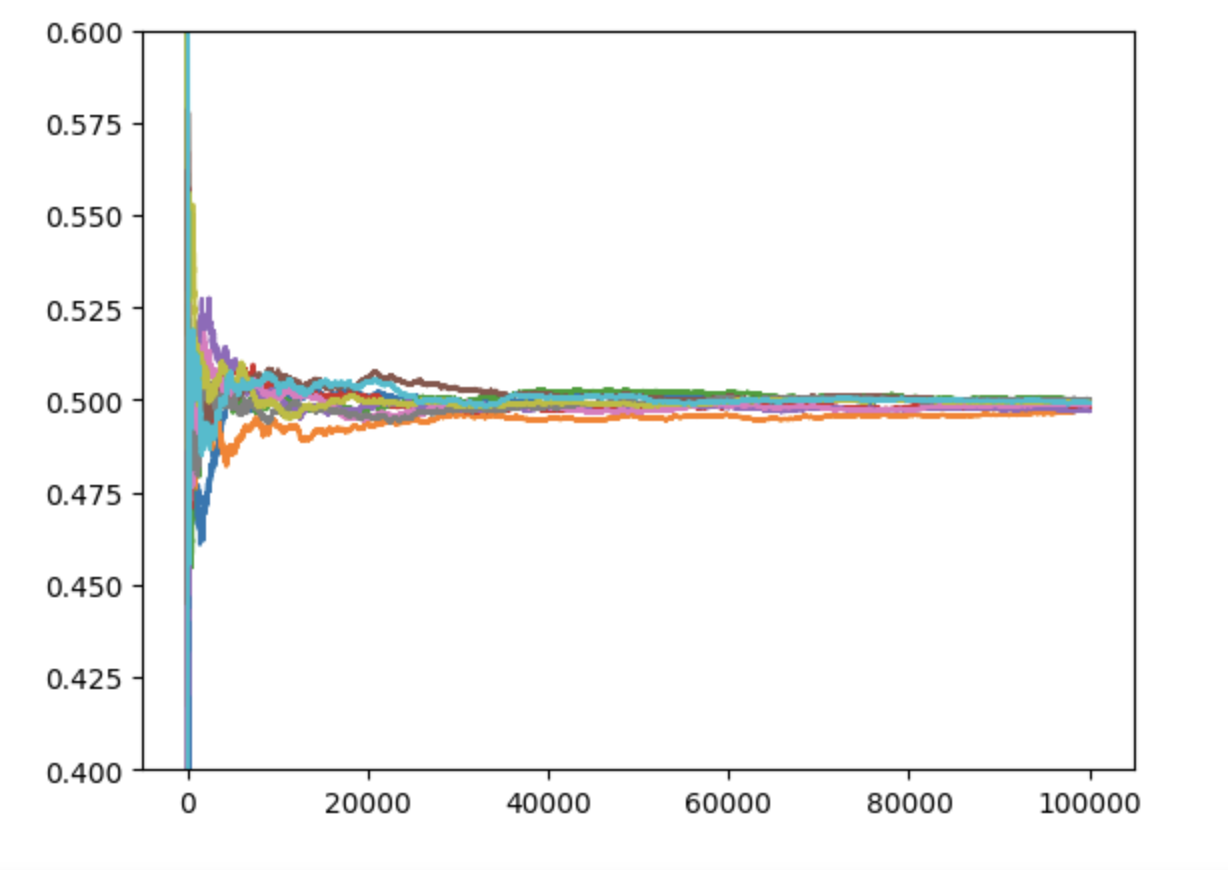
\includegraphics[scale=0.5]{convergence graph.png}
\end{figure}
The convergence graph shows what the winning probability of player A would be after these many times of simulation. From the line plot, we are able to see the graph converge to the value around 0.5 and become stable as the number of game increases. Thus we conclude that $10^6 $ a reasonable length for simulation. (We have tried 10 runs of $10^7$ games but would run pretty slow).
~\\\\
Central Limit Theorem states that if we sample many values from an unknown distribution and average them, and then do this multiple times, the average will be approximately normally distributed around the mean of the distribution.
We run 1000 times of 1000 games and plot a histogram to show the distribution of all probabilities we have when player A and B both use strategy 1. 
\begin{figure}[H]
\centering
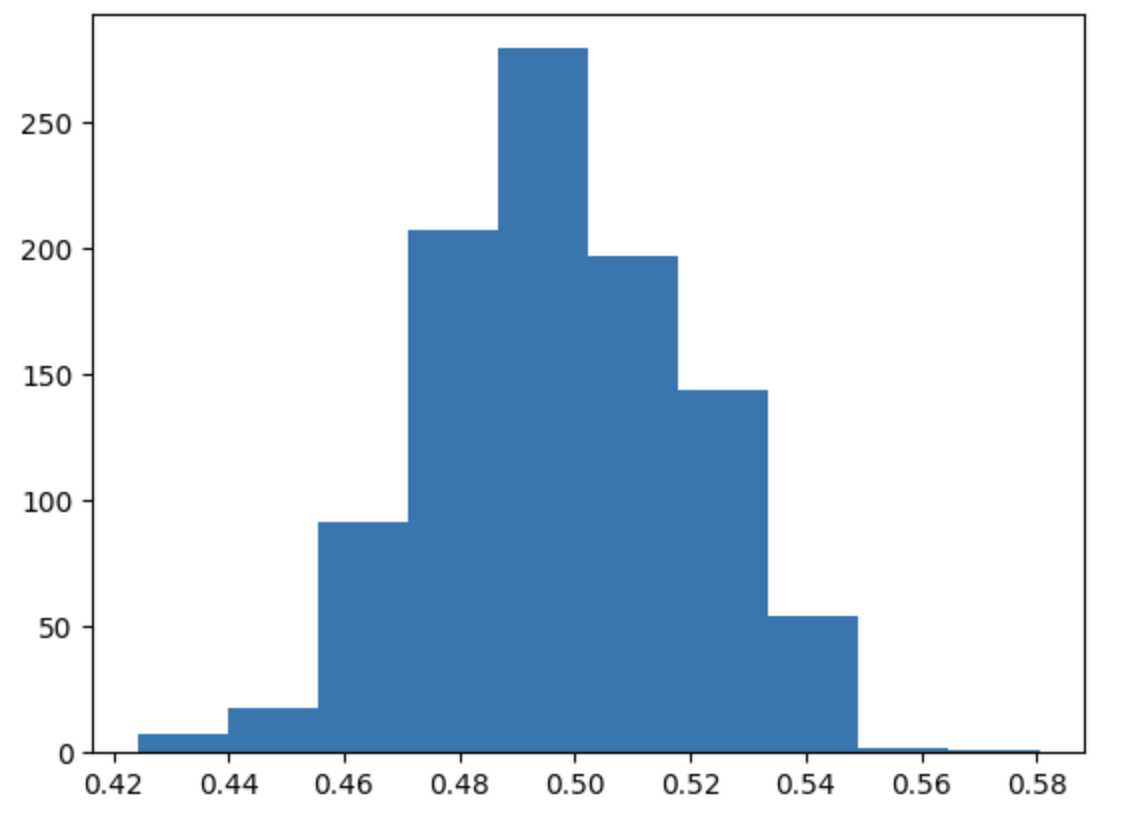
\includegraphics[scale=0.5]{histogram.png}
\end{figure}
As the Central Limit Theorem says and the histogram demonstrates, we can see that the distribution of probabilities is close to normally distributed.
If we use the fact that normally distributed implies symmetric about the mean, then we can estimate the probability that all 10 of our estimates are on one side of the true probability is:
\begin{align*}
    \frac{2}{2^{10}} \approx 0.001953125
\end{align*}
This explains the probability all the estimates are greater, or all of the estimates are less than the true probability. Therefore, we are 99.8\% confident that true winning probability will lie within the interval between lowest and highest estimate, that is, our confidence interval.
~\\\\
To better demonstrate the meaning of confidence interval, here is the results for players both use the first strategy as an example.\\
By running the simulation for 10 times, each time 10,0000 games will be played. In the following is the result of the win rate for player A:
$$\{ 0.50051\textit{ } 0.4973\textit{ }0.50158 \textit{ }0.49748 \textit{ }0.50028 \textit{ }0.49657 \textit{ }0.49921 \textit{ }0.50198 \textit{ }0.49762 \textit{ }0.49738 \}$$
\begin{table}[H]
  \begin{center}
    \begin{tabular}{|c|c|c|c|}
    \hline
    \textbf{Game round}
    & \textbf{Player A win} & \textbf{Player B win} & \textbf{tie} \\
    \hline
    1st run & 49746 & 50004 & 250\\
    \hline
    2nd run & 49595 & 50174 & 231\\
    \hline
    3rd run & 49761 & 50003 & 236\\
    \hline
    4st run & 49807 & 49947 & 246\\
    \hline
    5st run & 49835 & 49934 & 231\\
    \hline
    6st run & 50003 & 49776 & 221\\
    \hline
    7st run & 49914 & 49869 & 217\\
    \hline
    8st run & 49951 & 49820 & 229\\
    \hline
    9st run & 50017 & 49737 & 246\\
    \hline
    10st run & 49819 & 49948 & 233\\
    \hline
    \end{tabular}
  \end{center}
\end{table}
From these result we could see that the smallest win rate is 0.4973 and the largest win rate is 0.50198, thus it gives us 99.8\% confidence that the true probability would lies within the interval [0.4973 0.50198].

\section{Strategy Comparison and Analysis}
To see which strategy is more effective in helping the player have higher winning probability, or similarly, be highly confident that the true winning probability would lie in the confidence interval that is above 0.5, we operate pairwise comparisons of 5 strategies.\\\\
Here is the table showing what winning probability intervals would be for player A of each strategy compared with all the others.
\begin{table}[H]
  \begin{center}
  \caption*{Confidence Intervals of Winning Probability of Player A’s Strategy}
    \begin{tabular}{|c|c|c|c|c|c|c|}
    \hline
    \multirow{2}{*}{Player A} & \multicolumn{6}{c|}{Player B} \\
    \cline{2-7}
    & Strategy1 & Strategy2-5 & Strategy2-10 & Strategy3 &  Strategy4 & Strategy5\\
    \hline
    Strategy1 & [0.497, 0.502] & [0.470, 0.474]& [0.457, 0.463]& [0.159, 0.164] & [0.135, 0.138] & [0.066, 0.069]\\
    \hline
    Strategy2-5 & \color{red}[0.523, 0.530] & [0.496, 0.501]& [0.488, 0.497] & [0.217, 0.222] & [0.176, 0.180] & [0.109, 0.112]\\
    \hline
    Strategy2-10 & \color{red}[0.534, 0.542] & \color{red}[0.503, 0.508] & [0.492, 0.501] & [0.211, 0.219] & [0.179, 0.183] & [0.086, 0.089] \\
    \hline
    Strategy3 & \color{red}[0.834, 0.838] & \color{red}[0.778, 0.783] & \color{red}[0.778, 0.784] & [0.489, 0.499]& [0.406, 0.414] & [0.268, 0.273]\\
    \hline
    Strategy4 & \color{red}[0.859, 0.863] & \color{red}[0.818, 0.822]& \color{red}[0.817, 0.822] & \color{red}[0.572, 0.579] & [0.480, 0.488] & [0.418, 0.423]\\
    \hline
    Strategy5 & \color{red}[0.927, 0.933] & \color{red}[0.876, 0.882]& \color{red} [0.904, 0.906]& \color{red} [0.719, 0.727]& \color{red}[0.572, 0.578]& [0.468, 0.476]\\
    \hline
    \end{tabular}
  \end{center}
\end{table}
We may observe some symmetry in the table. For example, suppose $i$ and $j$ are a selected strategy among all 5. When two players take different strategies ($i \neq j$), the sum of confidence interval that if Player A takes Strategy $i$ and Player B takes Strategy $j$ ($i \neq j$) and confidence interval that if Player A takes Strategy $j$ and Player B takes Strategy $i$  would be approximately 1. \\\\
The elements highlighted in red demonstrate that if the player A takes certain strategy, would be more likely to win than choosing the strategy that Player B uses. Through comparisons, we are able to learn the overall ranking of 5 strategies:
(use '$>$' sign to symbolize if the strategy is better than the later one)
\begin{align*}
\text{Strategy} 5 > \text{Strategy} 4 > \text{Strategy} 3 > \text{Strategy} 2-10 > \text{Strategy} 2-5 > \text{Strategy} 1 
\end{align*}
Moreover, when comparing strategy 1 with every other strategies, both its lowest and highest estimate in the confidence interval are below 0.5 shown in the table. Thus, we could conclude the randomly play a game would be the worst choice when another player chooses to play wisely and strategically. \\
Strategy 5 is the most effective one. Instead of trusting luckiness totally and although Strategy 3 suggests comparing the current score above or below the goal, the strategy 4 is more practical and specific in deciding how many dices exactly to roll for winning. However, there would situation at certain roll, that for example the player reaches the score of 24. And at that condition, it would be wise to stop rolling since the total number of chances to win in the game is small as 3. So choose to not roll the dice whenever having the chance of super close to the goal 25. And this explains to some extent why Strategy 5 is the best choice. 
\section{Appendix}
Here is the Python code for simulation:\\
\url{https://colab.research.google.com/drive/1dIKudKMLehwYmLRZTyHwbH9AUiIzjziB?usp=sharing}

\end{document}

